\documentclass[journal,12pt,twocolumn]{IEEEtran}

\usepackage{setspace}
\usepackage{gensymb}

\singlespacing


\usepackage[cmex10]{amsmath}

\usepackage{amsthm}

\usepackage{mathrsfs}
\usepackage{txfonts}
\usepackage{stfloats}
\usepackage{bm}
\usepackage{cite}
\usepackage{cases}
\usepackage{subfig}

\usepackage{longtable}
\usepackage{multirow}

\usepackage{enumitem}
\usepackage{mathtools}
\usepackage{steinmetz}
\usepackage{tikz}
\usepackage{circuitikz}
\usepackage{verbatim}
\usepackage{tfrupee}
\usepackage[breaklinks=true]{hyperref}
\usepackage{graphicx}
\usepackage{tkz-euclide}
\usepackage{float}

\usetikzlibrary{calc,math}
\usepackage{listings}
    \usepackage{color}                                            %%
    \usepackage{array}                                            %%
    \usepackage{longtable}                                        %%
    \usepackage{calc}                                             %%
    \usepackage{multirow}                                         %%
    \usepackage{hhline}                                           %%
    \usepackage{ifthen}                                           %%
    \usepackage{lscape}     
\usepackage{multicol}
\usepackage{chngcntr}

\DeclareMathOperator*{\Res}{Res}

\renewcommand\thesection{\arabic{section}}
\renewcommand\thesubsection{\thesection.\arabic{subsection}}
\renewcommand\thesubsubsection{\thesubsection.\arabic{subsubsection}}

\renewcommand\thesectiondis{\arabic{section}}
\renewcommand\thesubsectiondis{\thesectiondis.\arabic{subsection}}
\renewcommand\thesubsubsectiondis{\thesubsectiondis.\arabic{subsubsection}}


\hyphenation{op-tical net-works semi-conduc-tor}
\def\inputGnumericTable{}                                 %%

\lstset{
%language=C,
frame=single, 
breaklines=true,
columns=fullflexible
}
\begin{document}


\newtheorem{theorem}{Theorem}[section]
\newtheorem{problem}{Problem}
\newtheorem{proposition}{Proposition}[section]
\newtheorem{lemma}{Lemma}[section]
\newtheorem{corollary}[theorem]{Corollary}
\newtheorem{example}{Example}[section]
\newtheorem{definition}[problem]{Definition}

\newcommand{\BEQA}{\begin{eqnarray}}
\newcommand{\EEQA}{\end{eqnarray}}
\newcommand{\define}{\stackrel{\triangle}{=}}
\bibliographystyle{IEEEtran}
\providecommand{\mbf}{\mathbf}
\providecommand{\pr}[1]{\ensuremath{\Pr\left(#1\right)}}
\providecommand{\qfunc}[1]{\ensuremath{Q\left(#1\right)}}
\providecommand{\sbrak}[1]{\ensuremath{{}\left[#1\right]}}
\providecommand{\lsbrak}[1]{\ensuremath{{}\left[#1\right.}}
\providecommand{\rsbrak}[1]{\ensuremath{{}\left.#1\right]}}
\providecommand{\brak}[1]{\ensuremath{\left(#1\right)}}
\providecommand{\lbrak}[1]{\ensuremath{\left(#1\right.}}
\providecommand{\rbrak}[1]{\ensuremath{\left.#1\right)}}
\providecommand{\cbrak}[1]{\ensuremath{\left\{#1\right\}}}
\providecommand{\lcbrak}[1]{\ensuremath{\left\{#1\right.}}
\providecommand{\rcbrak}[1]{\ensuremath{\left.#1\right\}}}
\theoremstyle{remark}
\newtheorem{rem}{Remark}
\newcommand{\sgn}{\mathop{\mathrm{sgn}}}
\providecommand{\abs}[1]{\left\vert#1\right\vert}
\providecommand{\res}[1]{\Res\displaylimits_{#1}} 
\providecommand{\norm}[1]{\left\lVert#1\right\rVert}
%\providecommand{\norm}[1]{\lVert#1\rVert}
\providecommand{\mtx}[1]{\mathbf{#1}}
\providecommand{\mean}[1]{E\left[ #1 \right]}
\providecommand{\fourier}{\overset{\mathcal{F}}{ \rightleftharpoons}}
%\providecommand{\hilbert}{\overset{\mathcal{H}}{ \rightleftharpoons}}
\providecommand{\system}{\overset{\mathcal{H}}{ \longleftrightarrow}}
	%\newcommand{\solution}[2]{\textbf{Solution:}{#1}}
\newcommand{\solution}{\noindent \textbf{Solution: }}
\newcommand{\cosec}{\,\text{cosec}\,}
\providecommand{\dec}[2]{\ensuremath{\overset{#1}{\underset{#2}{\gtrless}}}}
\newcommand{\myvec}[1]{\ensuremath{\begin{pmatrix}#1\end{pmatrix}}}
\newcommand{\mydet}[1]{\ensuremath{\begin{vmatrix}#1\end{vmatrix}}}
\numberwithin{equation}{subsection}
\makeatletter
\@addtoreset{figure}{problem}
\makeatother
\let\StandardTheFigure\thefigure
\let\vec\mathbf
\renewcommand{\thefigure}{\theproblem}
\def\putbox#1#2#3{\makebox[0in][l]{\makebox[#1][l]{}\raisebox{\baselineskip}[0in][0in]{\raisebox{#2}[0in][0in]{#3}}}}
     \def\rightbox#1{\makebox[0in][r]{#1}}
     \def\centbox#1{\makebox[0in]{#1}}
     \def\topbox#1{\raisebox{-\baselineskip}[0in][0in]{#1}}
     \def\midbox#1{\raisebox{-0.5\baselineskip}[0in][0in]{#1}}
\vspace{3cm}
\title{Assignment 6}
\author{K.A. Raja Babu}
\maketitle
\newpage
\bigskip
\renewcommand{\thefigure}{\theenumi}
\renewcommand{\thetable}{\theenumi}
Download all python codes from 
\begin{lstlisting}
https://github.com/ka-raja-babu/Matrix-Theory/tree/main/Assignment6/Codes
\end{lstlisting}
%
and latex-tikz codes from 
%
\begin{lstlisting}
https://github.com/ka-raja-babu/Matrix-Theory/tree/main/Assignment6
\end{lstlisting}
%
\section{Question No. 2.29}
Find the coordinates of the focus, axis, the equation of the directrix and latus rectum of the parabola $y^2$ = 8$x$ .
%
\section{Appendix}

All parameters of parabola $y^2=8x$ can be summarised in table \ref{tab:table1} .

Note : Given general formula is valid only when parabola is in standard form i.e. $\abs{\vec{V}}$ = 0 and $\lambda_1$ = 0 . 

$^{1}$ Procedure to find axis :
\begin{enumerate}
\item Calculate vertex $\vec{c}$ and focus $\vec{F}$.

\item Find equation of line joining $\vec{c}$ and $\vec{F}$ using           $\vec{x}=\vec{F} +k\vec{m}$ where $\vec{m}=\vec{F}-\vec{c}$ and $k \in \mathbb{R}.$
\end{enumerate}

$^{2}$ Procedure to find directrix :
\begin{enumerate}
\item Calculate its direction vector $\vec{v_1}$ by using $\vec{v}^T\vec{v_1} =        0.$
    \item Equate $\vec{v_1}^T\vec{x}$ to -$\beta$ to get final equation.
\end{enumerate}

$^{3}$ Procedure to find latus rectum :
\begin{enumerate}
\item Calculate its direction vector $\vec{v_2}$ by using $\vec{v}^T\vec{v_2} =        0.$
    \item Equate $\vec{v_2}^T\vec{x}$ to $\beta$ to get final equation.
\end{enumerate}

\numberwithin{table}{section}
\begin{table}[!ht]
\begin{center}
\begin{tabular}{ | m{1.4cm} | m{1.0cm}| m{2.4cm} | m{2.3cm} | } 
\hline
Para-\newline meter  & Sym-\newline bol  & Value  & General \newline Formula\\ 
\hline
Vertex & $\vec{c}$ & $\myvec{0\\0}$ & $\myvec{\vec{u}^T + \eta\vec{p_1}^T \\ \vec{V}}\vec{c}$ \newline $= \myvec{-f \\ \eta\vec{p_1} - \vec{u}}$ \\ 
\hline
Focal \newline Length & $\beta$ & 2 & $\frac{1}{4}\abs{\frac{2\eta}{\lambda_2}}$
\\ 
\hline
Focus & $\vec{F}$ & \myvec{2\\0} & $\vec{F}=\vec{c} + \vec{a}^T$ \\
\hline
Axis$^{1}$ &  & $\myvec{0 & 1}\vec{x}=0$ & $\vec{x}=\vec{F}+k\vec{m}$ \\
\hline
Axis di- \newline rection \newline vector & $\vec{v}$ & $\myvec{0 \\ 1}$ & $\vec{v}^T\vec{x}$ = 0 \\
\hline
Direct- \newline rix dire- \newline ction \newline vector & $\vec{v_1}$ & \myvec{1 \\ 0} & $\vec{v}^T\vec{v_1}$ = 0 \\
\hline
Direct- \newline rix$^{2}$ &  & $\myvec{1 & 0}\vec{x} = -2$ & $\vec{v_1}^T\vec{x} = -\beta$ \\
\hline
Latus \newline rectum \newline directi- \newline on vector & $\vec{v_2}$ & $\myvec{1 \\ 0}$ & $\vec{v}^T\vec{v_2}$ = 0 \\ 
\hline
Latus \newline rectum$^{3}$ & & $\myvec{1 & 0}\vec{x}=2$ & $\vec{v_2}^T\vec{x}=\beta$\\
\hline
End \newline points \newline of latus \newline rectum & $\vec{M},\vec{N}$ & $\myvec{2\\4},\myvec{2\\-4}$ & $\myvec{\beta \\ \pm y(\beta)}$ \\
\hline
Length \newline of latus \newline rectum & $l$ & 8 & $\norm{\vec{M}-\vec{N}}$\\
\hline
\end{tabular}
\end{center}
\caption{Parameters of parabola $y^2=8x$}
\label{tab:table1}
\end{table}

\clearpage
\begin{theorem}
General equation of a conic is given by
\begin{align}
ax^2+2bxy+cy^2+2dx+2ey+f=0 \label{eq:15}
\end{align}
and can be expressed as 
\begin{align}
    \vec{x}^T\vec{V}\vec{x} + 2\vec{u}^T\vec{x} + f = 0 \label{eq:1}
\end{align}
where
\begin{align}
    \vec{V}&=\vec{V}^T=\myvec{a & b\\b & c}
    \\
    \vec{u}&=\myvec{d & e}
\end{align}
\end{theorem}
\begin{theorem}
\eqref{eq:1} can be expressed as 
\begin{align}
    \vec{y}^T\vec{D}\vec{y} + 2(\vec{V}\vec{c} + \vec{u})^T \vec{P}\vec{y} + \vec{c}^T\vec{V}\vec{c} + 2\vec{u}^T\vec{c} + f = 0 \label{eq:22}
\end{align}
\end{theorem}
\begin{proof}
Using Affine Transformation,
\begin{align}
    \vec{x}=\vec{P}\vec{y}+\vec{c} \label{eq:2}
\end{align}
Using Eigenvalue Decomposition,
\begin{align}
    \vec{P}^T\vec{V}\vec{P}=\vec{D} \label{eq:4}
\end{align}
such that
\begin{align}
    \vec{D} &= \myvec{\lambda_1 & 0 \\ 0 & \lambda_2}
    \\
    \vec{P} &= \myvec{\vec{p_1} & \vec{p_2}},\hspace{0.5cm}
    \vec{P}^T = \vec{P}^{-1} \label{eq:5}
\end{align}
Substituting \eqref{eq:2} in \eqref{eq:1},we get
\begin{align}
    (\vec{P}\vec{y}+\vec{c})^T\vec{V}(\vec{P}\vec{y}+\vec{c}) + 2\vec{u}^T(\vec{P}\vec{y}+\vec{c}) + f = 0
\end{align}
which can be expressed as
\begin{multline}
\vec{y}^T\vec{P}^T\vec{V}\vec{P}\vec{y} + 2(\vec{V}\vec{c} + \vec{u})^T \vec{P}\vec{y}\\
+ \vec{c}^T\vec{V}\vec{c} + 2\vec{u}^T\vec{c} + f = 0 \label{eq:3}
\end{multline}

From \eqref{eq:3} and \eqref{eq:4},
\begin{align}
    \vec{y}^T\vec{D}\vec{y} + 2(\vec{V}\vec{c} + \vec{u})^T \vec{P}\vec{y} + \vec{c}^T\vec{V}\vec{c} + 2\vec{u}^T\vec{c} + f = 0
\end{align}
\end{proof}
\begin{theorem}
When $\abs{\vec{V}} = 0, \lambda_1 = 0$ and 
\begin{align}
\vec{V}\vec{p}_1 = 0, 
\vec{V}\vec{p}_2 = \lambda_2\vec{p}_2
\end{align}

Then, \eqref{eq:22} can be expressed as 
\begin{align}
\vec{y}^T\vec{D}\vec{y} = -2\eta\myvec{1 & 0}\vec{y} \label{eq:23}
\end{align}
\end{theorem}
\begin{proof}
Substituting \eqref{eq:5} in \eqref{eq:3},
\begin{multline}
\vec{y}^T\vec{D}\vec{y}+2\brak{\vec{c}^T\vec{V}+\vec{u}^T}\myvec{\vec{p}_1 & \vec{p}_2}\vec{y}
\\
+  \vec{c}^T\brak{\vec{V}\vec{c} + \vec{u}}+ \vec{u}^T\vec{c} + f= 0
\end{multline}
\begin{multline}
\implies
\vec{y}^T\vec{D}\vec{y}+2\myvec{\brak{\vec{c}^T\vec{V}+\vec{u}^T}\vec{p}_1 & \brak{\vec{c}^T\vec{V}+\vec{u}^T}\vec{p}_2}\vec{y}
\\
+  \vec{c}^T\brak{\vec{V}\vec{c} + \vec{u}}+ \vec{u}^T\vec{c} + f= 0
\end{multline}
\begin{multline}
\implies \vec{y}^T\vec{D}\vec{y}+2\myvec{\vec{u}^T\vec{p}_1 & \brak{\lambda_2\vec{c}^T+\vec{u}^T}\vec{p}_2}\vec{y}
\\
+  \vec{c}^T\brak{\vec{V}\vec{c} + \vec{u}}+ \vec{u}^T\vec{c} + f= 0
\end{multline}
\begin{multline}
\implies \lambda_2y_2^2+2\brak{\vec{u}^T\vec{p}_1}y_1+  2y_2\brak{\lambda_2\vec{c}+\vec{u}}^T\vec{p}_2
\\
+  \vec{c}^T\brak{\vec{V}\vec{c} + \vec{u}}+ \vec{u}^T\vec{c} + f= 0\label{eq:6}
\end{multline}
which is the equation of a parabola.

Thus,\eqref{eq:22} can be expressed as \eqref{eq:23} by choosing
\begin{align}
\eta = \vec{u}^T\vec{p}_1
\end{align}
such that
\begin{align}
\label{eq:7}
\vec{P}^{T}\brak{\vec{V}\vec{c}+\vec{u}} &= \eta\myvec{1\\0}
\\
\vec{c}^T\brak{\vec{V}\vec{c} + \vec{u}}+ \vec{u}^T\vec{c} + f&= 0
\label{eq:8}
\end{align}
\begin{align}
\therefore 
\vec{y}^T\vec{D}\vec{y} = -2\eta\myvec{1 & 0}\vec{y} \label{eq:11}
\end{align}
\end{proof}
\begin{lemma}
Focal length of a parabola is given by
\begin{align}
\beta = \frac{1}{4}\abs{\frac{2\vec{u}^T\vec{p}_1}{\lambda_2}} 
\label{eq:24} 
\end{align}
\end{lemma}
\begin{proof}
From \eqref{eq:6}, by comparing the coefficients of $y_2^2$ and $y_1$, the focal length of the parabola is obtained as 
\begin{align}
\beta = \frac{1}{4}\abs{\frac{2\vec{u}^T\vec{p}_1}{\lambda_2}} 
\label{eq:16} 
\end{align}
\end{proof}

\begin{lemma}
Vertex of a parabola when it is in standard form is given by 
\begin{align}
\myvec{\vec{u}^T + \eta\vec{p_1}^T \\ \vec{V}}\vec{c} = \myvec{-f \\ \eta\vec{p_1} - \vec{u}} \label{eq:28}
\end{align}
\end{lemma}
\begin{proof}
Multiplying \eqref{eq:7} by $\vec{P}$ yields
\begin{align}
\label{eq:9}
\brak{\vec{V}\vec{c}+\vec{u}} &= \eta\vec{p}_1,
\end{align}
which, upon substituting in \eqref{eq:8}
results in 
\begin{align}
\eta\vec{c}^T\vec{p}_1 + \vec{u}^T\vec{c} + f&= 0
\label{eq:10}
\end{align}
\eqref{eq:9} and \eqref{eq:10} can be clubbed together to obtain 
\begin{align}
\myvec{\vec{u}^T + \eta\vec{p_1}^T \\ \vec{V}}\vec{c} = \myvec{-f \\ \eta\vec{p_1} - \vec{u}} \label{eq:12}
\end{align}
\end{proof}

\begin{lemma}
Focus of a parabola when it is in standard form is given by 
\begin{align}
\vec{a} &= \frac{-2\eta\myvec{1 & 0}}{4} 
\\
\vec{F} &= \vec{c} + \vec{a}^T  \label{eq:25}
\end{align}
\end{lemma}
\begin{proof}
From \eqref{eq:11},focus $\vec{F}$ can be calculated as
\begin{align}
\vec{a} &= \frac{-2\eta\myvec{1 & 0}}{4} 
\\
\vec{F} &= \vec{c} + \vec{a}^T  \label{eq:13}
\end{align}
\end{proof}
\begin{definition}
Axis  of  a parabola  always passes through  both  vertex and focus \label{def:1}
\end{definition}
\begin{lemma}
Axis of a parabola when it is standard form is given by
\begin{align}
    \vec{x} &= \vec{F}+k\vec{m} \quad \brak{k \in \mathbb{R}} \label{eq:26}
\end{align}
\end{lemma}
\begin{proof}
Using definition \ref{def:1}, axis can be calculated by finding equation of line joining vertex and focus.
\\
Using $\vec{c}$ from \eqref{eq:12} and $\vec{F}$ from \eqref{eq:13},
\\
axis can be calculated as
\begin{align}
\vec{m} &= \vec{F}-\vec{c} \quad (\text{$\vec{m}$ is direction vector})
\\
\vec{x} &= \vec{F}+k\vec{m} \quad \brak{k \in \mathbb{R}} \label{eq:14}
\\
\implies \vec{v}^T\vec{x} &= 0 \quad (\text{$\vec{v}$ is direction vector of $\vec{x}$}) \label{eq:21}
\end{align}
\end{proof}
\begin{definition}
Vertex  of  parabola  is  at  equal  distance  from focus and directrix and directrix is perpendicular to axis. \label{def:2}
\end{definition}
\begin{lemma}
Directrix of a parabola when it is in standard form is given by
\begin{align}
    \vec{v_1}^T\vec{x} = -\beta 
\end{align}
\end{lemma}
\begin{proof}
Using definition \ref{def:2},directrix is always perpendicular to axis such that
\begin{align}
\vec{v}^T\vec{v_1} = 0 \quad (\text{$\vec{v_1}$ is direction vector of directrix}) \label{eq:19}
\end{align}
Using \eqref{eq:16} and \eqref{eq:19},directrix can be expressed as 
\begin{align}
    \vec{v_1}^T\vec{x} = -\beta 
\end{align}
\end{proof}
\begin{definition}
Latus rectum of parabola passes through focus and is perpendicular to axis. \label{def:3}
\end{definition}
\begin{lemma}
Latus rectum of a parabola when it is in standard form is given by 
\begin{align}
    \vec{v_2}^T\vec{x} = \beta 
\end{align}
\end{lemma}
\begin{proof}
Using definition \ref{def:3},latus rectum is always perpendicular to axis such that
\begin{align}
    \vec{v}^T\vec{v_2} = 0 \quad (\text{$\vec{v_2}$ is direction vector of latus rectum}) \label{eq:20}
\end{align}
Using \eqref{eq:16} and \eqref{eq:20},latus rectum can be expressed as 
\begin{align}
    \vec{v_2}^T\vec{x} = \beta 
\end{align}
\end{proof}
\begin{lemma}
End points of latus rectum of a parabola when it is in standard form is given by
\begin{align}
    \vec{M}&=\myvec{\beta \\ y(\beta)} 
    \\
    \vec{N}&=\myvec{\beta \\ -y(\beta)} 
\end{align}
\end{lemma}
\begin{proof}
Using \eqref{eq:15} and \eqref{eq:16},end points of latus rectum can be expressed as 
\begin{align}
    \vec{M}&=\myvec{\beta \\ y(\beta)} \label{eq:17}
    \\
    \vec{N}&=\myvec{\beta \\ -y(\beta)} \label{eq:18}
\end{align}
\end{proof}

\begin{lemma}
Length of latus rectum is given by 
\begin{align}
    l=\norm{\vec{M}-\vec{N}}
\end{align}
\end{lemma}
\begin{proof}
Using \eqref{eq:17} and \eqref{eq:18},length of latus rectum can be expressed as
\begin{align}
    l=\norm{\vec{M}-\vec{N}}
\end{align}
\end{proof}

\section{solution}
Given parabola is 
\begin{align}
y^2 &= 8x
\\
\implies y^2 - 8x &= 0
\end{align}

Vector form of given parabola is
\begin{align}
\vec{x}^T\myvec{0 & 0 \\ 0 & 1}\vec{x} + 2\myvec{-4 & 0}\vec{x} + 0 &= 0 
\end{align}

$\therefore$
\begin{align}
 \vec{V} = \myvec{0 & 0 \\ 0 & 1} ,
 \vec{u} = \myvec{-4\\0} ,
 f = 0
\end{align}

$\because$
$|\vec{V}|$ = 0 and $\lambda_1$ = 0 i.e. it is in standard form
\\
$\therefore$
\begin{align}
\vec{P}=\vec{I} \implies \vec{p_1} = \myvec{1\\0}
\\
\eta = \vec{u}^T\vec{p_1} = -4
\end{align}

The vertex $\vec{c}$ is given by
\begin{align}
\myvec{-8 & 0\\0 & 0\\0 & 1}\vec{c} &= \myvec{0\\0\\0}
\\
\implies \vec{c} &= \myvec{0\\0}
\end{align}

The focal length $\beta$ is given by
\begin{align}
\beta = \frac{1}{4}\abs{\frac{2\eta}{\lambda_2}} = \frac{1}{4}\abs{\frac{-8}{1}}= 2
\end{align}

The focus $\vec{F}$ is given by
\begin{align}
\vec{a} &= \frac{-2\eta\myvec{1 & 0}}{4} = \myvec{2 & 0}
\\
\vec{F} &= \vec{c} + \vec{a}^T = \myvec{2\\0}
\end{align}

$\because$
Axis of parabola passes through both vertex and focus .
\\
$\therefore$
Axis of parabola is given by
\begin{align}
\vec{m} =\vec{F} - \vec{c} &= \myvec{2\\0}
\\
\vec{x} = \vec{F} + k\vec{m} &= \myvec{2+2k \\ 0}
\\
\implies \myvec{0 & 1}\vec{x} &= 0
\\
\implies \vec{v} = \myvec{0 \\ 1}
\end{align}

$\because$
Vertex of parabola is at equal distance from focus and directrix and directrix is perpendicular to axis.
\\
$\therefore$
Directrix of parabola is given by
\begin{align}
\vec{v}^T\vec{v_1} = 0
\\
\implies \vec{v_1} = \myvec{1 \\ 0}
\end{align}
So , 
\begin{align}
\vec{v_1}^T\vec{x} = -\beta
\\
\implies \myvec{1 & 0}\vec{x} = -2
\end{align}

$\because$
Latus rectum of parabola passes through focus and is perpendicular to axis.
\\
$\therefore$
Latus rectum of parabola is given by
\begin{align}
\vec{v}^T\vec{v_2} = 0
\\
\implies \vec{v_2} = \myvec{1 \\ 0}
\end{align}
So , 
\begin{align}
\vec{v_2}^T\vec{x} = \beta
\\
\implies \myvec{1 & 0}\vec{x} = 2
\end{align}

End points of latus rectum are
\begin{align}
\vec{M} &= \myvec{2\\4}
\\
\vec{N} &= \myvec{2\\-4}
\end{align}

So,the length of latus rectum $l$ is 
\begin{align}
l = \norm{\vec{M}-\vec{N}} = 8
\end{align}
\newpage
Plot of given parabola

\numberwithin{figure}{section}
\begin{figure}[!ht]
\centering
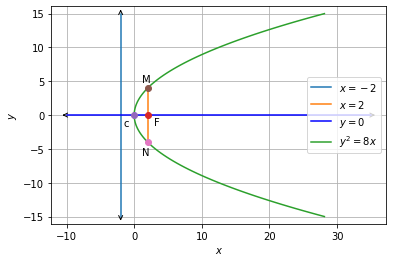
\includegraphics[width=\columnwidth]{Figure6}
\caption{Parabola $y^2=8x$ }
\label{fig:parabola}	
\end{figure}

\end{document}
